% ===============================================================
% =							Related Work 						=
% ===============================================================
\chapter{Results and Evaluation}
\label{cha:results}

To experiment the results of our tool, we took various approaches as for testing. In this chapter we describe the methods and results of the tests and inquiries on a group of users.

\section{Algorithm Comparison}

Since we decided to use modified version of some algorithms to use them in a real-time environment, it made sense to compare our results with ones obtained from the original algorithms. 
One the algorithms we used that was partially implemented, was the object segmentation (Section \ref{sub:segmentation}). For this algorithm we opted for not using Grabcut \cite{rother2004grabcut} to refine the results since the saliency map already gave a good indication of what was the object in a scenario.  To compare with the original algorithm, we used the same dataset as the author and compared the resulting segmentation masks.

From a subset of 500 images from the original dataset, we ran our implementation and could conclude that for almost all the images, a significant part of the main subject in the photo was always detected. Since we decided not to use Grabcut, our results could not be refined and therefore our segmentation mask would have a lot of unfilled areas that were still considered as part of the subject. In other cases, the saliency map that we implemented completely failed. Some of the reasons for this to fail was the lack of contrast of the subject in comparison to the background or because the background had higher contrast. Another thing that highly influences the results is the brightness because bright areas were more likely to be chosen as part of the subject.

As referred in Section \ref{sub:segmentation}, our segmentation mask was based on pixels that were considered as foreground while all other were background. In an attempt to fill the areas that were not considered foreground and still belonged to the subject, we considered all pixels as foreground since they were inside of a bounding area. We also did a comparison of the method with the original algorithm using the same subset of images. 
For the tested images, it fulfilled its purpose. However, in most images it ruins the results because many background elements are then added to the mask. Some of the results can be seen and compared in Annex \ref{app:seg_results}.


Another algorithm we tested, was the colour template detection. For this feature we implemented a simpler algorithm instead of simplifying the original one. However, \citeauthor{cohen2006color} \cite{cohen2006color} didn't describe any methods of evaluation for this algorithm. We then used a couple of images that showed results and compared the results of our own algorithm. In Annex \ref{app:temp_results} it is possible to observe some images used by the author and compare the results obtained from the original algorithm with our results. From what we could conclude, our results were not to far from the expected and still give a good indication if the colour is using a monochromatic or complementary template, and what are the most salient colours.


The last algorithm we compared was the horizon detection algorithm. We gathered 32 images from Flickr that were labelled with the tags \emph{seascape}, \emph{landscape} and \emph{horizon}, as this were likely to have a clear horizon line and some with obstructed horizon. The result was evaluated by comparing the position and angle of the detected horizon line with a manually-annotated horizon line. For each image, the position of the horizon line was calculated by averaging the vertical position of the two points forming the line, and used the same two points to calculate the slope of the line then converted to an angle. In Annex \ref{app:horizon_results} are the results obtained from the images tested. We could verify that in the images labelled as \emph{seascape} and \emph{landscape} the deviation of the horizon position was relatively low with only an average relative error of 9.5\% and 8.2\%. On the contrary, images labelled as \emph{horizon}, had an average relative error of 55\%, due to being images more prominent to edges. However, for the angles, there is a high deviation in most of the values. This is because the values of the angles are very close to zero, thus the difference between the calculated value and the original one is almost neglectible but has high impact in the relative error for being a division of two very small numbers. In most cases, the angle difference between the real horizon line and the detected horizon line is small and doesn't really affect the judgement of where the horizon line is.

\section{Algorithm Execution Time}

Having the purpose of displaying information in real-time, we considered that the execution times of each algorithm should be taken into account. Algorithms with a slow performance are less likely to be useful in a real-time scenario and might even ruin the experience of the user. With that in mind, we did performance tests over each feature to understand its reliability in real-time processing.


\subsection{Testing tool}
These times were taken by generating log files that contain trace information to analyse. We used the Android's \emph{Debug} class to call the methods \emph{startMethodTracing()} and \emph{stopMethodTracing()}, to start and stop logging of trace information to disk. This option is very precise because we can specify exactly where to start and stop logging trace data in your code. For all tests we started the profile in the moment that the application receives a frame from the device's camera, and stopped right after processing that frame and refresh the view of the current feature \cite{SDK}.

After generating the log files, we used a tool called \emph{dmtracedump} to generate a graphical call-stack diagram from the trace log files. Figure \ref{fig:trace_ex} illustrates an example of the generated diagram from a trace file. 
In this tree diagram each call is represented as a node, and shows the call flow (from parent node to child node) using arrows. For each node, \emph{dmtracedump} shows \emph{<ref> callname (<inc-ms>, <exc-ms>,<numcalls>)}, where

\begin{itemize}
\item \emph{<ref>} - Call reference number, as used in trace logs,
\item \emph{<inc-ms>} - Inclusive elapsed time (milliseconds spent in method, including all child methods),
\item \emph{<exc-ms>} - Exclusive elapsed time (milliseconds spent in method, not including any child methods),
\item \emph{<numcalls>} - Number of calls.
\end{itemize}

\begin{figure}[htb]
	\centering
	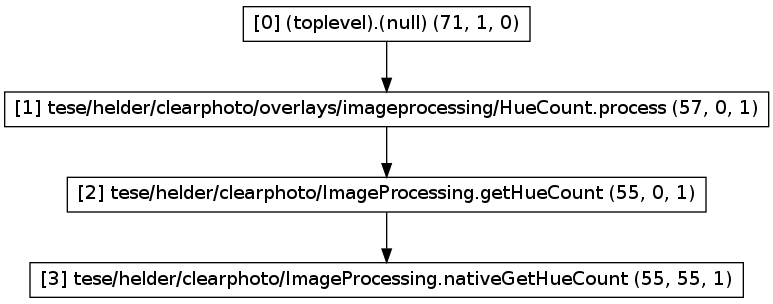
\includegraphics[width=\textwidth]{interface/trace.png}
	\caption{Graphical diagram generated from a trace log file.}
	\label{fig:trace_ex}
\end{figure}

Using the trace log file and these diagrams, we were able to get the amount of milliseconds spent in a method and any method called by it (\emph{<inc-ms>}), and the total time it took to perform the computation from the start to finish.
For each feature we took 10 samples and ignored the lowest and highest value to then calculate the average time and standard deviation for the total amount of time it took to perform the trace and the time spent in the method that processed the data. This way we expect to obtain relevant information about the time spent processing the frame and refreshing the view of each feature.

\subsection{Results}

All the times taken are in Annex \ref{app:exec_times} represented by a table with the time of each sample and the average of total time spent.
Some of these features where tested under different conditions or parameters to understand the difference in performance. For example, the saturation detection (Table \ref{tab:sat}) was tested in scenarios where the detector successfully indicated low saturation and in scenarios where it failed. We could conclude by the samples taken that the detector performs better when it fails to detect a low saturation environment. This is due to the extra computational effort that the device has to make to convert the frame into grayscale to display on the viewfinder. However the algorithm is not that heavy and it still performs quite well, disregarding the visual cue that can easily be replaced by a more appropriate one.

Another feature that we experimented in different scenarios was the face detection (Table \ref{tab:face}). We experimented detecting one or three faces as well as using the suggestions for improving the composition. As we can conclude from the results, there weren't any significant changes from each one the scenarios. As expected, the most costly computation was the detection of a face in a frame. In comparison, the calculation of the suggestion to improve the composition is neglectable.

The detection of main lines is dependent of a threshold, therefore we sampled the algorithm with different thresholds. The threshold values tested were 160, 100 and 40 as lower thresholds detect more lines. As we can conclude from Table \ref{tab:major_lines}, for all thresholds the computational effort was similar regardless of the threshold.

We also implemented three algorithms to calculate the simplicity on an image, therefore, the performance of each one was tested individually (Table \ref{tab:simplicity}). We could conclude that the fastest method was the second method described by \citeauthor{kaoautomatic} \cite{kaoautomatic}. However, as discussed in Section \ref{subsub:simp_disc}, this is the least reliable method comparing to the other two. On the other end, the first method \cite{luo2008photo} and the third method \cite{ke2006design} tested are slower but more reliable. Being approximately 50ms slower, any of these methods is a good option.

From the remaining features, the ones that performed better were the histograms calculation, detection of templates and scoring based on the \emph{Hue} channel. For the sampled tests, all these features performed in 50-150ms which can be translated into 6~20 frames-per-second, where the colour histogram in the \emph{Hue} channel and colour template detection had the slowest times. 

On the other end, the slowest feature were the object segmentation, the image balance and the detection of the horizon line, with average times of approximately 240ms, 600ms and 2700ms, respectively. Being more complex algorithms, these results were expected. However, detecting the image balance and the horizon line, are algorithms too demanding to be used on a real-time scenario. Object segmentation and horizon line detection are algorithms that give important visual feedback since they work as an overlay over the real frame, however both algorithms perform poorly.

These tests were performed in Samsung Galaxy Note with Android 4.1. We made sure that each feature was doing what was expected of it for at least 30 seconds, so that the results would be the most reliable possible. After that, we extracted the log files from the mobile device and extracted the execution time for each run, from a total of 10 runs.
 
\section{Users Testing}

The evaluation of this proof-of-concept tool was made by conducting functionality tests study to 10 users. The test was composed of a set of basic tasks and questionnaire. In some cases, it led to a discussion with more experienced test subjects. The tasks were focused on getting an assessment about the utility and overall satisfaction on the functionalities implemented and try to understand if they are useful in a real-time scenario. The questionnaires consisted in a total of 47 questions using the Likert scale (1-\emph{strongly disagree} to 5-\emph{strongly agree}) and an area for suggestions and comments about what was experienced. During the evaluation tests, a Samsung Galaxy Note was used for the application.

\subsection{Participants}

As mentioned before, we did tests to a total of 10 subjects of both genders, with 64\% males and 36\% females. The ages varied through 22 and 24, being the predominant age 23 with 50\% of the users. To understand what kind of background the users had, we realized a couple of questions to assess their knowledge of photography. We could conclude that 10 (91\%) of the test subjects take photographs but 7 (64\%) had any knowledge in the area and all of them classified their level of knowledge as amateur. When asked about what kind of devices to take photographs, the majority answered camera phones (75\%). Some still admitted to use still cameras (27\%), instant cameras (18\%) and DSLR cameras (18\%). The frequency of use of each device can be seen in Figure \ref{fig:q6} (Annes \ref{app:questionnaire_results}).

\subsection{Questionnaire}

For the questionnaires, we asked the users to test all the functionalities and answer a total of 47 questions using the Likert scale. The users started by experimenting the features related to colour information. 

When asked about the \emph{RGB} histogram, we could conclude that the tests subjects considered the feature useful (Figure \ref{fig:q10}). When asked if it gave a good idea of the range of colours being used and if the purpose of the dynamic bar was clear, we obtained a positive feedback (Figure \ref{fig:q7} and \ref{fig:q9}). However, we observed during the tests that the purpose of the line indicating the amount of pixels near the boundaries was not well understood and that could be verified by the results ($Mo = 3$) in Figure \ref{fig:q8}.

Regarding to the histogram implementation using the \emph{Hue} channel, the results were positive. The users strongly agreed that the number of colours in the spectrum to be adequate (Figure \ref{fig:q11}) and that in this representation would be easy to see the most used colour and its complementary to balance the image (Figure \ref{fig:q12}). However, when asked about its usefulness and if it gave a good idea of the colours being used, the average of responses was \emph{agree} (Figure \ref{fig:q13} and \ref{fig:q14}). We were expecting \emph{strongly agree}, as we though it would be much useful in comparison to regular histograms since it gave more realistic information regarding the colours being used.

We could observe that many test subjects had difficulty in understanding the saturation detection. Although they mostly answered \emph{agree} when asked if indicated the usage of a monochromatic filter and its usefulness (Figure \ref{fig:q15} and \ref{fig:q16}), we could detect that there were difficulties in understanding the concept of the feature and how to try it out. We already discussed in Section \ref{subsub:disc_hist} that it would be difficult to find real-world scenarios to test this feature, and that could be verified during the testing stage.

About the colour template detector, the average of votes went to \emph{agree} when asked about this feature usefulness and if the difference between between scenarios with a monochromatic or complementary colour schemes (Figure \ref{fig:q19} and \ref{fig:q20}). However, we had low results when we asked if the colour scale was adequate, with many of the users answering \emph{neutral} (Figure \ref{fig:q17}).

When asked about the hue scoring feature considered the feature combined well with the colour template detector and that it would reflect the simplicity of the scenario (Figure \ref{fig:q23} and \ref{fig:q24}). Since it was considered to reflect the simplicity, the users also \emph{agreed} that it was useful (Figure \ref{fig:q22}) which was the main concern in this feature. However, most of the test subjects responded \emph{neutral} when asked if the scale used was adequate (Figure \ref{fig:q21}). 

Face detection is something that is already implemented in multiple photographing devices nowadays. We obtained very positive answers when we asked about the usefulness of using face detection with grids, exploring the triangular composition and rule of the odds (Figure \ref{fig:q25}, \ref{fig:q25} and \ref{fig:q25}). Overall, the test subjects mostly choose \emph{strongly agree} when asked if this feature was useful. We considered this feature to have the problem of showing too much information, however, many of the test subjects disagree as we can see in Figure \ref{fig:q29}.

For the horizon detection, most users \emph{agreed} that the detector gave the correct result and it was useful (Figure \ref{fig:q31} and \ref{fig:q33}). Being used in a real-time environment, we considered the performance to be an important part of these set of tools. When asked about if it performed well in real-time, the test subjects confirmed that this feature as a poor performance and is to heavy to be used in this conditions (Figure \ref{fig:q32}).

When asked about the detection of prominent lines, the results were pretty average. The test subjects \emph{agreed} to be useful, the resulting lines corresponded to the leading lines in the scenario and that the visual cue would facilitate its usage in a composition (Figure \ref{fig:qmainline}).

Compared to all the other features, the object segmentation received the lowest scores. The test subjects responded \emph{neutral}, when asked about its usefulness and if the result was accurate (Figure \ref{fig:q37} and \ref{fig:q38}). These answers were somewhat expected since the algorithm would need specific conditions to work well, such as having an object with a salient colour over a a simple background.

For the image simplicity feature, the test subjects gave the same scoring has the other features regarding its usefulness (Figure \ref{fig:q44}). When asked if visual representation through bars or numbers, the users considered the bars to be better (Figure \ref{fig:q39} and \ref{fig:q40}). Since we implemented three different algorithms, we also asked about its results. The user considered the first implementation \cite{luo2008photo} to have the most accurate results (Figure \ref{fig:q41}). The other two algorithms \cite{kaoautomatic,ke2006design} received the same score even though we considered the algorithm by \citeauthor{ke2006design} \cite{ke2006design} had the best results of all three implementations (Figure \ref{fig:q42} and \ref{fig:q43}).

In the end the user had to test the image balance feature. We had to explain to some test subjects what consisted this feature, as it was not obvious to everyone. The questionnaires results show that the users mostly \emph{agreed} when asked if the symmetry axis was accurate, if the result was the expected and if it was useful (Figure \ref{fig:qimagebalance}).

In the end we received positive feedback in most of the features. Although not perfect, some tests subjects considered the tools useful, specially the detector of prominent lines, the image simplicity detector and the histogram using the \emph{Hue} channel.
We also received a couple of critiques. Although, the interface was not our main concern, some users suggested that it should give more hints on what each feature actually does. For someone who does not have knowledge in photography, they might not take much benefit of these tools, and for that to happen it would be needed to implement an interface able to give useful hints about each one. The algorithms were considered to be too slow which caused the user to be impatient. Many of the times, we could verify that the user didn't knew if it had to wait for a result. It was suggested to give a feedback while the algorithm is being run.
One of the users suggested to use this features after the photo was taken to analyse and improve the photo, becoming useful in the learning of how to take photographs.